\textbf{Un pescador est\'a sobre un oc\'eano rectangular. El valor del pez en el punto $(i, j)$ est\'a dado por un arreglo A de dimensi\'on 2 $n \times m$. Dise\~na un algoritmo que calcule el m\'aximo valor de pescado que un pescador puede atrapar en un camino desde la esquina superior izquierda a la esquina inferior derecha. El pescador solo puede moverse hacia abajo o hacia la derecha, como se ilustra en la siguiente figura.}\vspace{.2cm}

\begin{figure}[H]
    \centering
    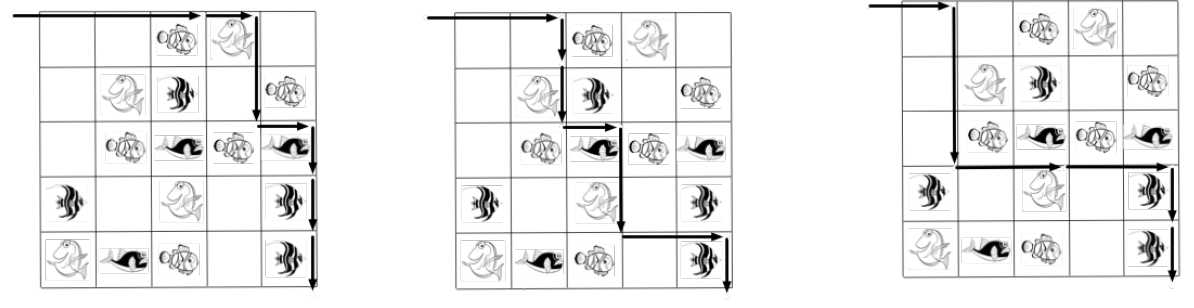
\includegraphics[width=0.75\linewidth]{src/Img/lago.PNG}
\end{figure}

\textcolor{bibi}{}
\begin{quote}
\end{quote}